\section{Моделирование когерентного MIMO радиолокатора}\label{sect:mimo-modeling}

Рассмотрим структуру модели MIMO радиолокатора второго вида (по классификации из \cite{li2008mimo}),
также называемого когерентным MIMO радаром.

Модель проводит симуляцию для $N$ передающих элементов расположенных линейно вдоль оси
$Ox$ и $M$ приёмных, расположенных вдоль оси $Oy$.

\begin{figure}[H]
    \centering
    \begin{subfigure}[b]{0.49\textwidth}
        \centering
        \hspace*{-3ex}
        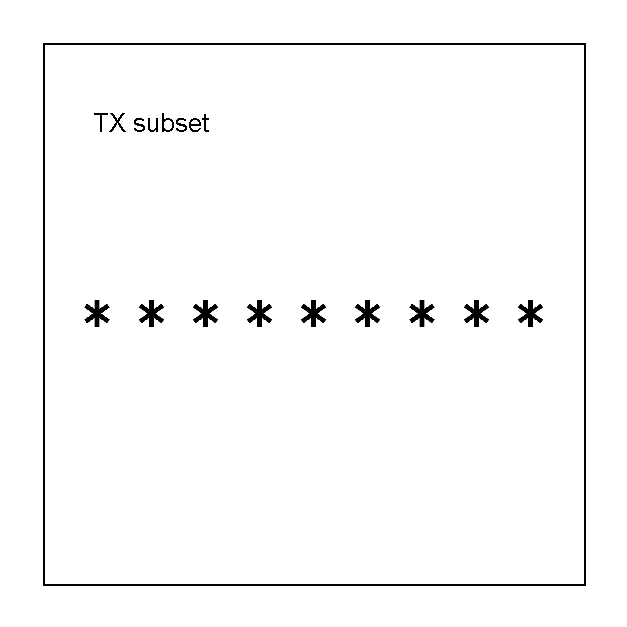
\includegraphics[width=\textwidth]{MIMO-TX}
        \caption{}%
    \end{subfigure}
    \hfill
    \begin{subfigure}[b]{0.49\textwidth}
        \centering
        \hspace*{-3ex}
        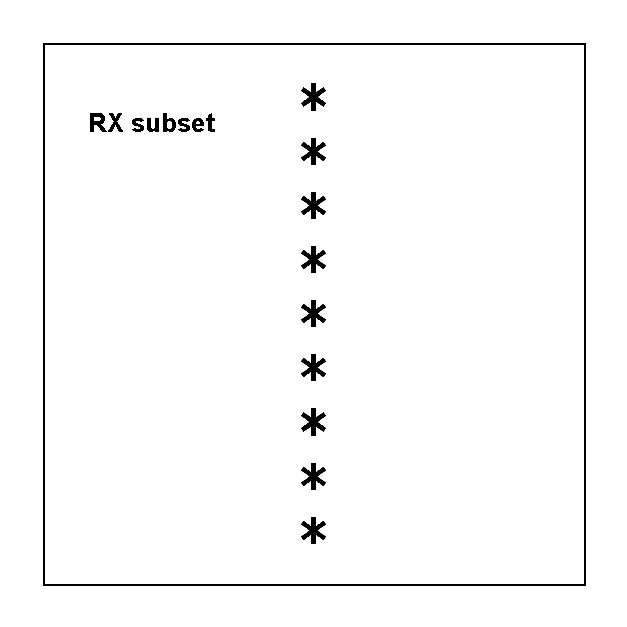
\includegraphics[width=\textwidth]{MIMO-RX}
        \caption{}%
    \end{subfigure}
    \caption{положения антенных элементов}%
    \label{fig:mimo-elemnt-pos}
\end{figure}


В результате совместной обработки будет получена виртуальная решётка, показанная на Рисунке~\ref{fig:mimo-virtual-array}.

\begin{figure}[H]
    \centering
    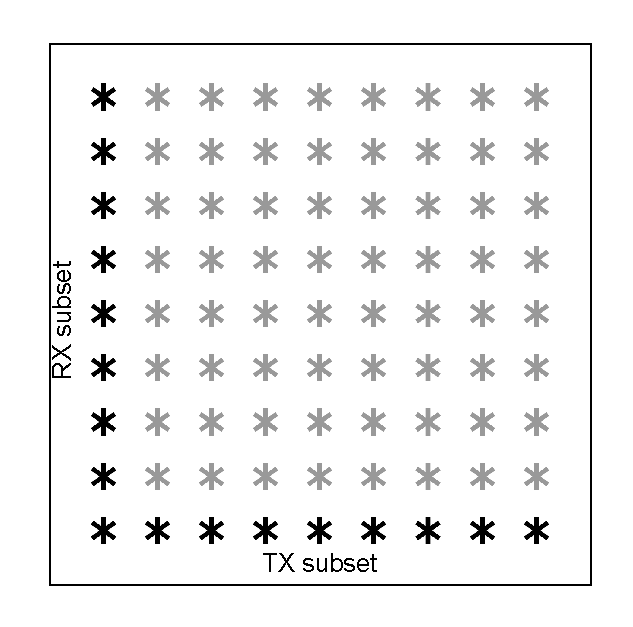
\includegraphics[width=0.8\textwidth,height=0.35\textheight,keepaspectratio]{MIMO-Virtual}
    \caption{Геометрия синтезированной антенной решётки. Виртуальные элементы отмечены серым цветом}%
    \label{fig:mimo-virtual-array}
\end{figure}

Входными данными в программу симуляции являются координаты цели в сферических координатах
с началом в центре виртуальной решётки.

В Таблице~\ref{table:mimo-model-parameters} приведены параметры целей, которые будут обнаруживаться в процессе симуляции.


\begin{table}[H]
    \centering
    \begin{tabular}{|c|c|c|}
        \hline
        $R$, м & $\theta$, град & $\phi$, град \\ \hline
        1500   & 20             & 25           \\ \hline
        1000   & -20            & -25          \\ \hline
    \end{tabular}
    \caption{Параметры целей}\label{table:mimo-model-parameters}
\end{table}

Работа программы моделирования состоит из следующих этапов:

\begin{enumerate}
    \item Задание параметров АР
    \item Генерация М-последовательностей для каждого элемента передающей решётки. 
    \item Модуляция передаваемых сигналом с помощью BPSK. Модуляция происходит с помощью комплексной экспоненты на нулевой частоте.
    \item Расчёт сигналов, излучаемых передающей решёткой и принятых на i-той цели
    \item Расчёт и сложение комплексных сигналов, отражённых от целей, и принятых на приёмной решётке
    \item Проведение свёртки по дальности для каждой отдельной M-последовательности. Формирование виртуальной АР
    \item Расчёт ДН для каждой дальности
    \item Обработка ДН, удаление сигналов меньше определённой амплитуды
    \item Сведение всех дальностей в общую плоскость решений
\end{enumerate}

Результат работы программы показан на Рисунке~\ref{fig:mimo-modeling-result}. 
Исходный код программы приведён в Приложении~\ref{appendix:mimo-modeling-appendix}.


\begin{figure}[H]
    \centering
    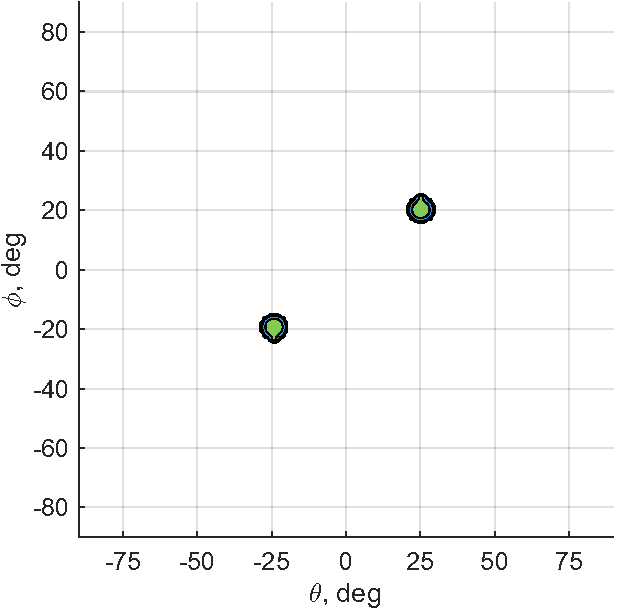
\includegraphics[width=0.8\textwidth,height=0.4\textheight,keepaspectratio]{mimo-modeling-result}
    \caption{Результаты моделирования MIMO радиолокатора}%
    \label{fig:mimo-modeling-result}
\end{figure}

\subsection{Заключение}

MIMO радиолокаторы обладают следующими преимуществами:

\begin{itemize}
    \item Компактность -- антенны MIMO радаров обладают меньшими размерами по сравнению с классическими АФАР,
    ввиду меньшего количества антенных элементов 
    \item Адаптивная цифровая обработка -- так как все вычисления проходят в цифровой части радиолокатора, 
    адаптивная обработка сигналов, в частности, подавление помех и формирование сложных ДНА, 
    может быть выполнена более качественно. 
    \item Увеличение угловой разрешающей способности -- возможности ЦАР по формировании более подходящих 
    для данных задач коэффициентов, позволяет MIMO радиолокаторам достигать 
    более высокой разрешающей способности по сравнению с классическими АФАР и SIMO радарами с тем же количеством элементов.
    \item Увеличение разрешающей способности и чувствительности при детектировании движущихся целей -- 
    MIMO радары лучше обнаруживают медленно движущиеся цели, чем классические АФАР с тем же количеством элементов
    \item Реконфигурируемость -- технические характеристики MIMO радаров связаны с возможностями обрабатывающей 
    техники. Вычислительные процессоры совершенствуются каждый год, 
    предлагая увеличение производительности от 10~до~50\% по сравнению с прошлыми реализациями. 
    Улучшить возможности MIMO радаров по формированию многолучевых ДН, активному сопровождению целей и 
    идентификации направления прихода сигнала можно за счёт обновления только системы обработки, 
    тогда как более дорогая аналоговая часть будет оставаться неизменной
\end{itemize}

В то же время они обладают следующими недостатками:

\begin{itemize}
    \item Сложность проектирования систем обработки -- MIMO радары генерируют большое количество данных. 
    Необходимо успевать обрабатывать текущий набор данных до того как придёт следующий, 
    что требует проектирования более сложной программной архитектуры и 
    параллельных цифровых аппаратных обработчиков данных
    \item Синхронизация между каналами -- для эффективной работы радара необходимо очень точно 
    синхронизировать тактовые сигналы как между каналами одного типа, 
    так и между приёмниками и передатчиками. 
    Влияние рассинхронизации на точность результатов подробно описаны в работе \cite{bondarenko2011affection}.
    \item Сложность детектирования быстродвижущихся целей
\end{itemize}

Тем не менее, исследования MIMO радаров активно ведутся, предлагая новые, более эффективные архитектуры и 
методы обработки сигналов. 
На текущий момент MIMO радары являются передовой областью в радарной технике. 
Однако их повсеместное внедрение связано с рядом технических и практических вызовов: сложность и стоимость таких систем,
требования к энергопотреблению и необходимость проектирования 
мощных систем обработки принятых данных являются преградами к их применению. 

Таким образом можно заключить, что MIMO радары обладают большим потенциалом, 
однако их массовое внедрение может произойти только по прошествию 
нескольких лет развития современной вычислительной техники.
